\documentclass[13pt]{beamer}
\usepackage[utf8]{inputenc}
\usepackage[T1]{fontenc}
\usepackage{lmodern}
\usepackage[english]{babel}
\usetheme{Marburg}
\usepackage{amsmath}
\usepackage{amsfonts}
\usepackage{amssymb}
\usepackage{graphicx}
\usepackage{tikz}
\usepackage{siunitx}

\begin{document}
	\author{Gabriel Gomes}
	\title{A Concise Introduction to Fuzzy Time Series}
	\subtitle{and practical applications in Santos Port}
	\institute{FATEC-RL}
	\date{}
	
	\begin{frame}[plain]
		\maketitle{}
	\end{frame}
	
	\begin{frame}
		\begin{center}
			\Large \textit{``All models are wrong, but some are useful.''} \newline
			\normalsize	-George E. P. Box
		\end{center}
	\end{frame}
	
	\begin{frame}
		\frametitle{Overview}
		\framesubtitle{Topics of this presentation:}
		\begin{itemize}
			\item<1-1> Fuzzy Logic — What it is and how it started?
			\item<2-2> Fuzzy Time Series — The main idea.
			\item<3-3> Santos Port — Time series characteristics.
			\item<4-4> Fuzzy Time Series and Simple Linear Regression — What Your Model Assumes Before You Start.
		\end{itemize}
	\end{frame}
	
	\begin{frame}
		\frametitle{Overview}
		\framesubtitle{Topics of this presentation:}
		\begin{itemize}
			\setlength{\itemsep}{2em}
			\item Fuzzy Logic — What it is and how it started?
			\item Fuzzy Time Series — The main idea. 
			\item Santos Port — Time series characteristics.
			\item Fuzzy Time Series and Simple Linear Regression — What Your Model Assumes Before You Start.
		\end{itemize}
	\end{frame}
	
	\begin{frame}{Fuzzy Logic}
		\framesubtitle{What is and how it started?}
		\begin{block}{ }
			\begin{tikzpicture}[remember picture, overlay]
				\node[anchor=east, outer sep=5pt] at (current page.east) {
					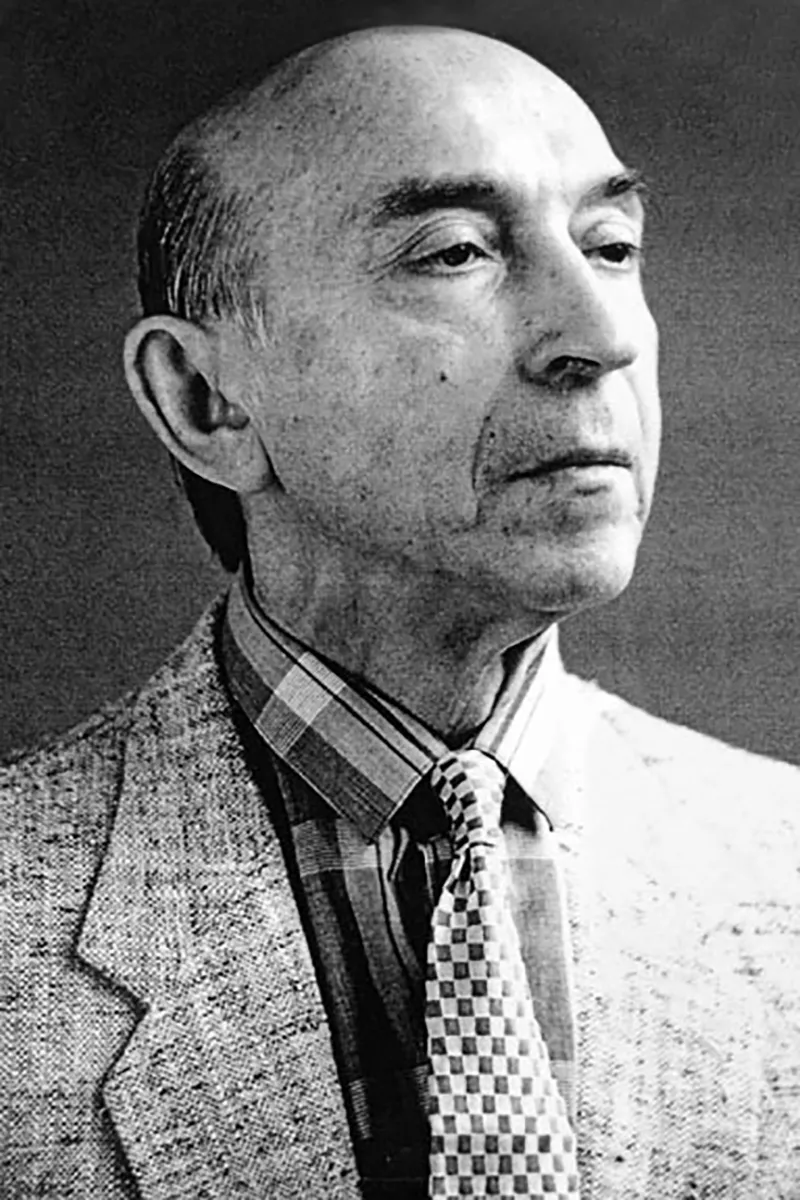
\includegraphics[width=1.7cm]{Images/Roberts-Lotfi-Zadeh.jpg}
				};
			\end{tikzpicture}
			Fuzzy theory was introduced in 1965 by Lotfi A. Zadeh, he published his paper in the Journal "Information and Control" with the title "Fuzzy Sets".
		\end{block}
		
		\begin{figure}
			\centering
			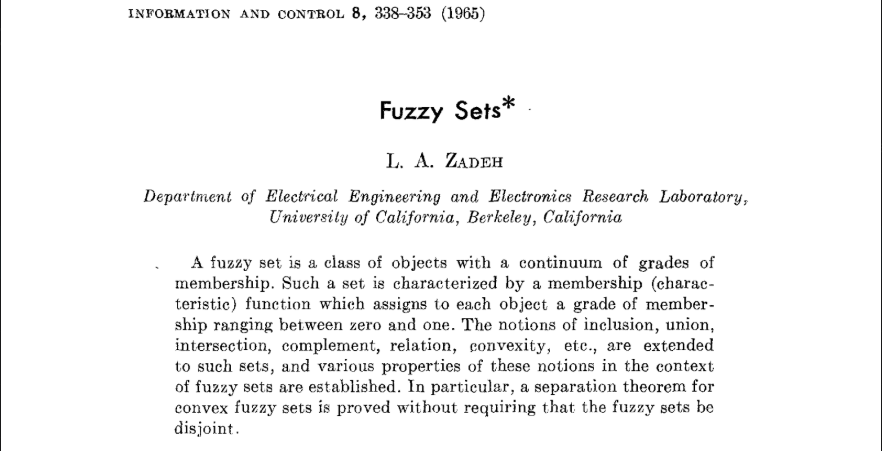
\includegraphics[width=0.9\textwidth]{Images/FSets.png} 
		\end{figure}
		
	\end{frame}
	
	\begin{frame}
		\frametitle{Dealing with subjectiveness in ordinal qualitative variables:}
		
		When speaking of variables, we usually classify them as:
		\newline
		\begin{itemize}
			\setlength{\itemsep}{1em}
			\item Quantitative: Variables that we can make mathematical operations and obtain statistical values such as mean, median, standard deviation... 
			\item Qualitative: They express non-numerical characteristics, such as attributes and labels, which can be of 2 types, nominal or ordinal. 
		\end{itemize}
		
	\end{frame}
	
	\begin{frame}
		Let's take ordinal variables in 2 examples: 
		\newline \newline
		A hierarchical degree of instruction levels (e.g. bachelor degree, master degree, Ph.D.) and a subjective variable such as hot, warm, cold.
		\newline \newline
		The distinction from both lies in the crispness of the boundaries: instruction levels have well-defined categorical thresholds, while terms like 'hot' or 'warm' admit gradual, overlapping membership, a structure that classical set theory cannot capture.
	\end{frame}
	
	
	\begin{frame}
		\frametitle{Ordinal Encoding of Instruction Levels}
		
		\begin{columns}[T]
			\begin{column}{0.45\textwidth}
				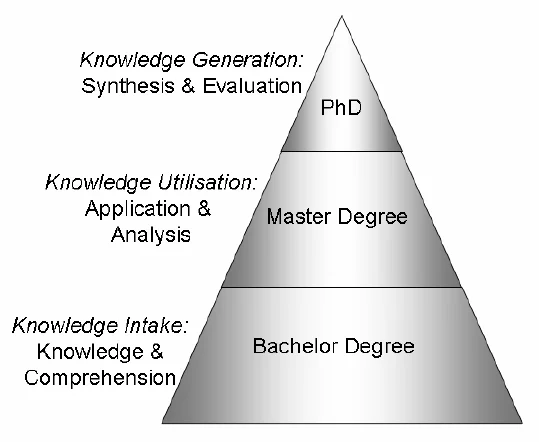
\includegraphics[width=\linewidth]{Images/degree.png}
			\end{column}
			\begin{column}{0.55\textwidth}
				\vspace{0.5em}
				The levels of instruction can be encoded in a computational
				way, with a direct ``cut'' and proper separation of the states,
				without affecting the substantial perception we have from it.
			\end{column}
		\end{columns}
		
		\vspace{2em}
		
		\textbf{Ordinal Encoding:} \quad
		$\text{Bachelor} = 1 \quad \text{Master} = 2 \quad \text{Ph.D.} = 3$
		
		\vspace{2em}
		
		{\small \textit{Note: this encoding preserves order only —
				arithmetic operations on these values are structurally undefined.}}
		
	\end{frame}
	
	
	\begin{frame}
		The problem begins when we have to deal with categories that are purely linguistic and pass this sense of graduality into a computer. That's why in fuzzy sets we work with the membership function which is a mathematical generalization of a indicator function in classical sets.
		
		\begin{table}[]
			\centering
			\begin{tabular}{c|c}
				Binary & Fuzzy \\ \hline
				$\mu$ $\in$ $ \{ 0,1 \} $ & $\mu$ $\in$ $[0,1]$
			\end{tabular}
		\end{table}
		
		We cannot classify hot as \SI{30}{\degreeCelsius} and assume that below this value is warm, because \SI{29}{\degreeCelsius} is much closer to hot than it is to warm. In order to compute precisely a value between hot and warm we can make a fuzzy inference system (FIS) based on the process conceptualized by Mamdani in 1975.
		
	\end{frame}
	
	\begin{frame}{Fuzzy Inference System}
		\framesubtitle{An applied example of fuzzy theory:}
		
		FIS is a framework based on a process of fuzzy logic rules that allow us to compute ordinal qualitative variables with human experience based-knowledge:
		
		\begin{figure}
			\centering
			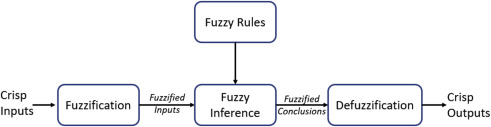
\includegraphics[width=0.6\textwidth]{Images/FIS2.jpg} 
		\end{figure}
		
		\begin{figure}
			\centering
			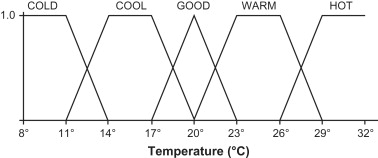
\includegraphics[width=0.6\textwidth]{Images/FIS.jpg} 
		\end{figure}
		
		In our example \SI{29}{\degreeCelsius} would belong to an intersection between warm and hot membership, giving us an output of how much would be in the both instances.
		
	\end{frame}
	
	\begin{frame}{Fuzzy Logic - What it is and how it started?}
		\framesubtitle{Conclusions:}
		
		\textbf{In a simplified way:} Fuzzy Logic can mathematically and computationally approximate the subjectiveness that we know of those variables. \newline
		
		So far we worked with a type of static data without temporal dependency, but the problem of modeling with fuzzy logic shifts when we have a time series data. \newline
		
		A time series is a collection of data from a variable distributed on a given period of time, by that we are not analyzing individually some data, we now have values that the current position is set by its $n$ preceding values:
		
		\begin{equation}
			x_t = f(x_{t-1}, x_{t-2}, ..., x_{t-n})
		\end{equation}
		
	\end{frame}
	
	\begin{frame}{Fuzzy Time Series}
		\framesubtitle{The main idea}
		
		Introduced in 1993 by Song and Chissom in their seminal paper "Fuzzy time series and its models", this new forecasting method based on Zadeh's work has implemented a way to use linguistic variables in a time series to forecast future values by a series of Fuzzy Logic Relations.
		
		\begin{figure}
			\centering
			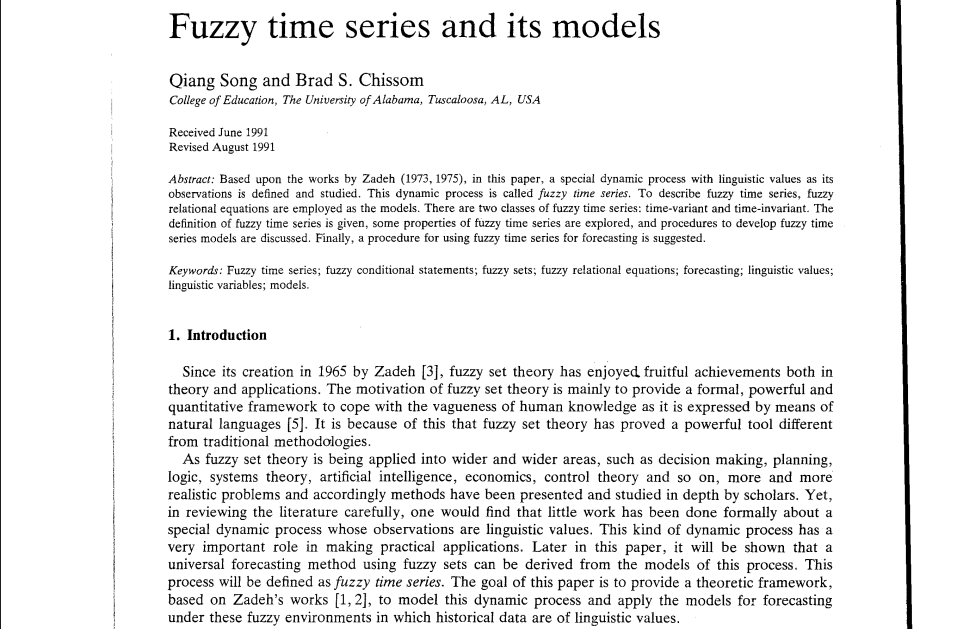
\includegraphics[width=0.8\textwidth]{Images/FTS.png} 
		\end{figure}
		
	\end{frame}
	
	\begin{frame}{Fuzzy Time Series}
		\framesubtitle{The main idea}
		
		Unfortunately, their first model presentation required complex matrix calculations due to max-min composition operations, and that changed when the simplified version of Chen (1996) using basic arithmetic, turned accessible and widely popular the FTS method.
		
		\begin{table}[]
			\centering
			\renewcommand{\arraystretch}{1.2}
			\resizebox{\columnwidth}{!}{%
				\begin{tabular}{l|c|c}
					& \textbf{Song \& Chissom (1993)} & \textbf{Chen (1996)} \\ \hline
					\textbf{Relation} 
					& $R = \bigcup_{i=1}^{n} A_{i}^{\top} \times A_{i+1}$ 
					& RLF Groups for current stage \\ \hline
					\textbf{Forecasting} 
					& $A_i = A_{i-1} \circ R$ 
					& $\hat{y}_{i+1} = \frac{1}{p}\sum_{k=1}^{p} m_k$
				\end{tabular}%
			}
		\end{table}
		
	\end{frame}
	
	\begin{frame}{Chen Method}
		
		% Alters the sub-item marker from a triangle to a circle
		\setbeamertemplate{itemize subitem}[circle] 
		
		Chen's method has been one of the simplest Fuzzy Time Series model, and it goes as the following steps: 
		\vspace{0.5em} % Adds a subtle breath before the list begins
		
		\begin{itemize}
			\setlength{\itemsep}{1.2em} % Expands the distance between primary nodes
			
			\item Define the linguistic variable
			\begin{itemize}
				\item Define Universe of Discourse and number of partitions
				\item Data Partitioning method 
				\item Create a fuzzy set for each partition
			\end{itemize}
			
			\item Fuzzification
			\begin{itemize}
				\item Fuzzy Time Series data
			\end{itemize}
			
			\item Formulate FLR and FLRG
			\begin{itemize}
				\item Fuzzy temporal patterns
				\item Fuzzy rules
			\end{itemize}
			
			\item Defuzzification
			\begin{itemize}
				\item Generate non-fuzzy outputs
			\end{itemize}
			
		\end{itemize}
	\end{frame}
	
	\begin{frame}
		Definition: \quad Let $Y(t)$, $t = 0, 1, 2, \dots$, be a time series whose Universe of Discourse is a subset of $\mathbb{R}$, on which fuzzy sets $A_i$, $i = 1, 2, \dots, k$ are defined. Let $F(t)$ consist of a sequence of fuzzified values of $Y(t)$. Then, $F(t)$ is called a fuzzy time series defined on $Y(t)$, $t = 0, 1, 2, \dots$
		
		\begin{figure}
			\centering
			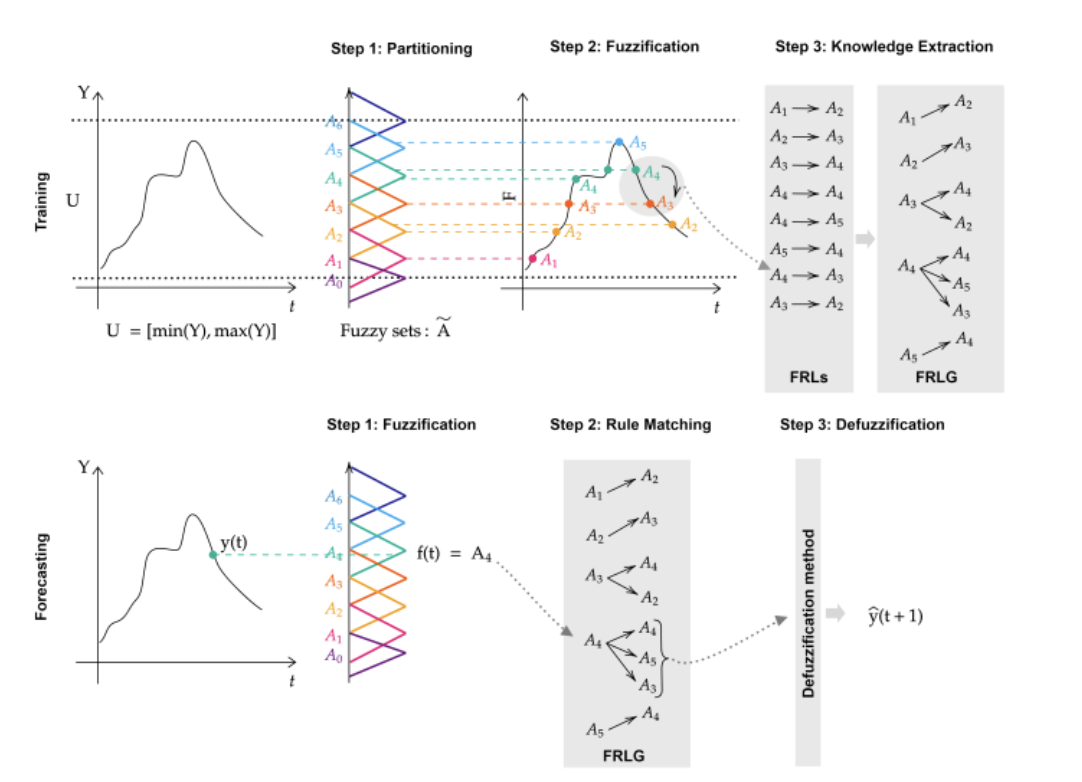
\includegraphics[width=1\linewidth]{Images/FTS_Process.png}
		\end{figure}
		
	\end{frame}
	
	\begin{frame}{Fuzzy Logic Group Relation (FLRG)}
		Each rule $\mathcal{R}_i \in \mathcal{R}$ has the format $LHS \rightarrow RHS$:
		
		\begin{itemize}
			\item $L^p A_{ip}, \dots, L A_{i1} \rightarrow A_{j1}, A_{j2}, \dots, A_{jn}$, where $L X_t = X_{t-1}$
			\item $LHS = \{L^p A_{ip}, \dots, L A_{i1}\}$ is used to match the input patterns
			\item $RHS = \{A_{j1}, A_{j2}, \dots, A_{jn}\}$ is used to forecast the future values
		\end{itemize}
	\end{frame}
	
	\begin{frame}
		Once the rules have been obtained, they form the knowledge base of the model. \newline
		
		The forecasting procedure is:
		
		\setbeamertemplate{itemize subitem}[circle] 
		
		\vspace{0.5em} % Adds a subtle breath before the list begins
		
		\begin{itemize}
			\setlength{\itemsep}{1.2em} % Expands the distance between primary nodes
			
			\item Fuzzification
			\begin{itemize}
				\item Fuzzify the input Y(t)
			\end{itemize}
			
			\item Find active fuzzy rules
			\begin{itemize}
				\item Match the fuzzified input with the LHS of the rules in the knowledge base
			\end{itemize}
			
			\item Defuzzification
			\begin{itemize}
				\item Generate non-fuzzy forecasting value
			\end{itemize}
		\end{itemize}
		
		
		
	\end{frame}
	
	\begin{frame}{Many FTS Models}
		\begin{figure}
			\centering
			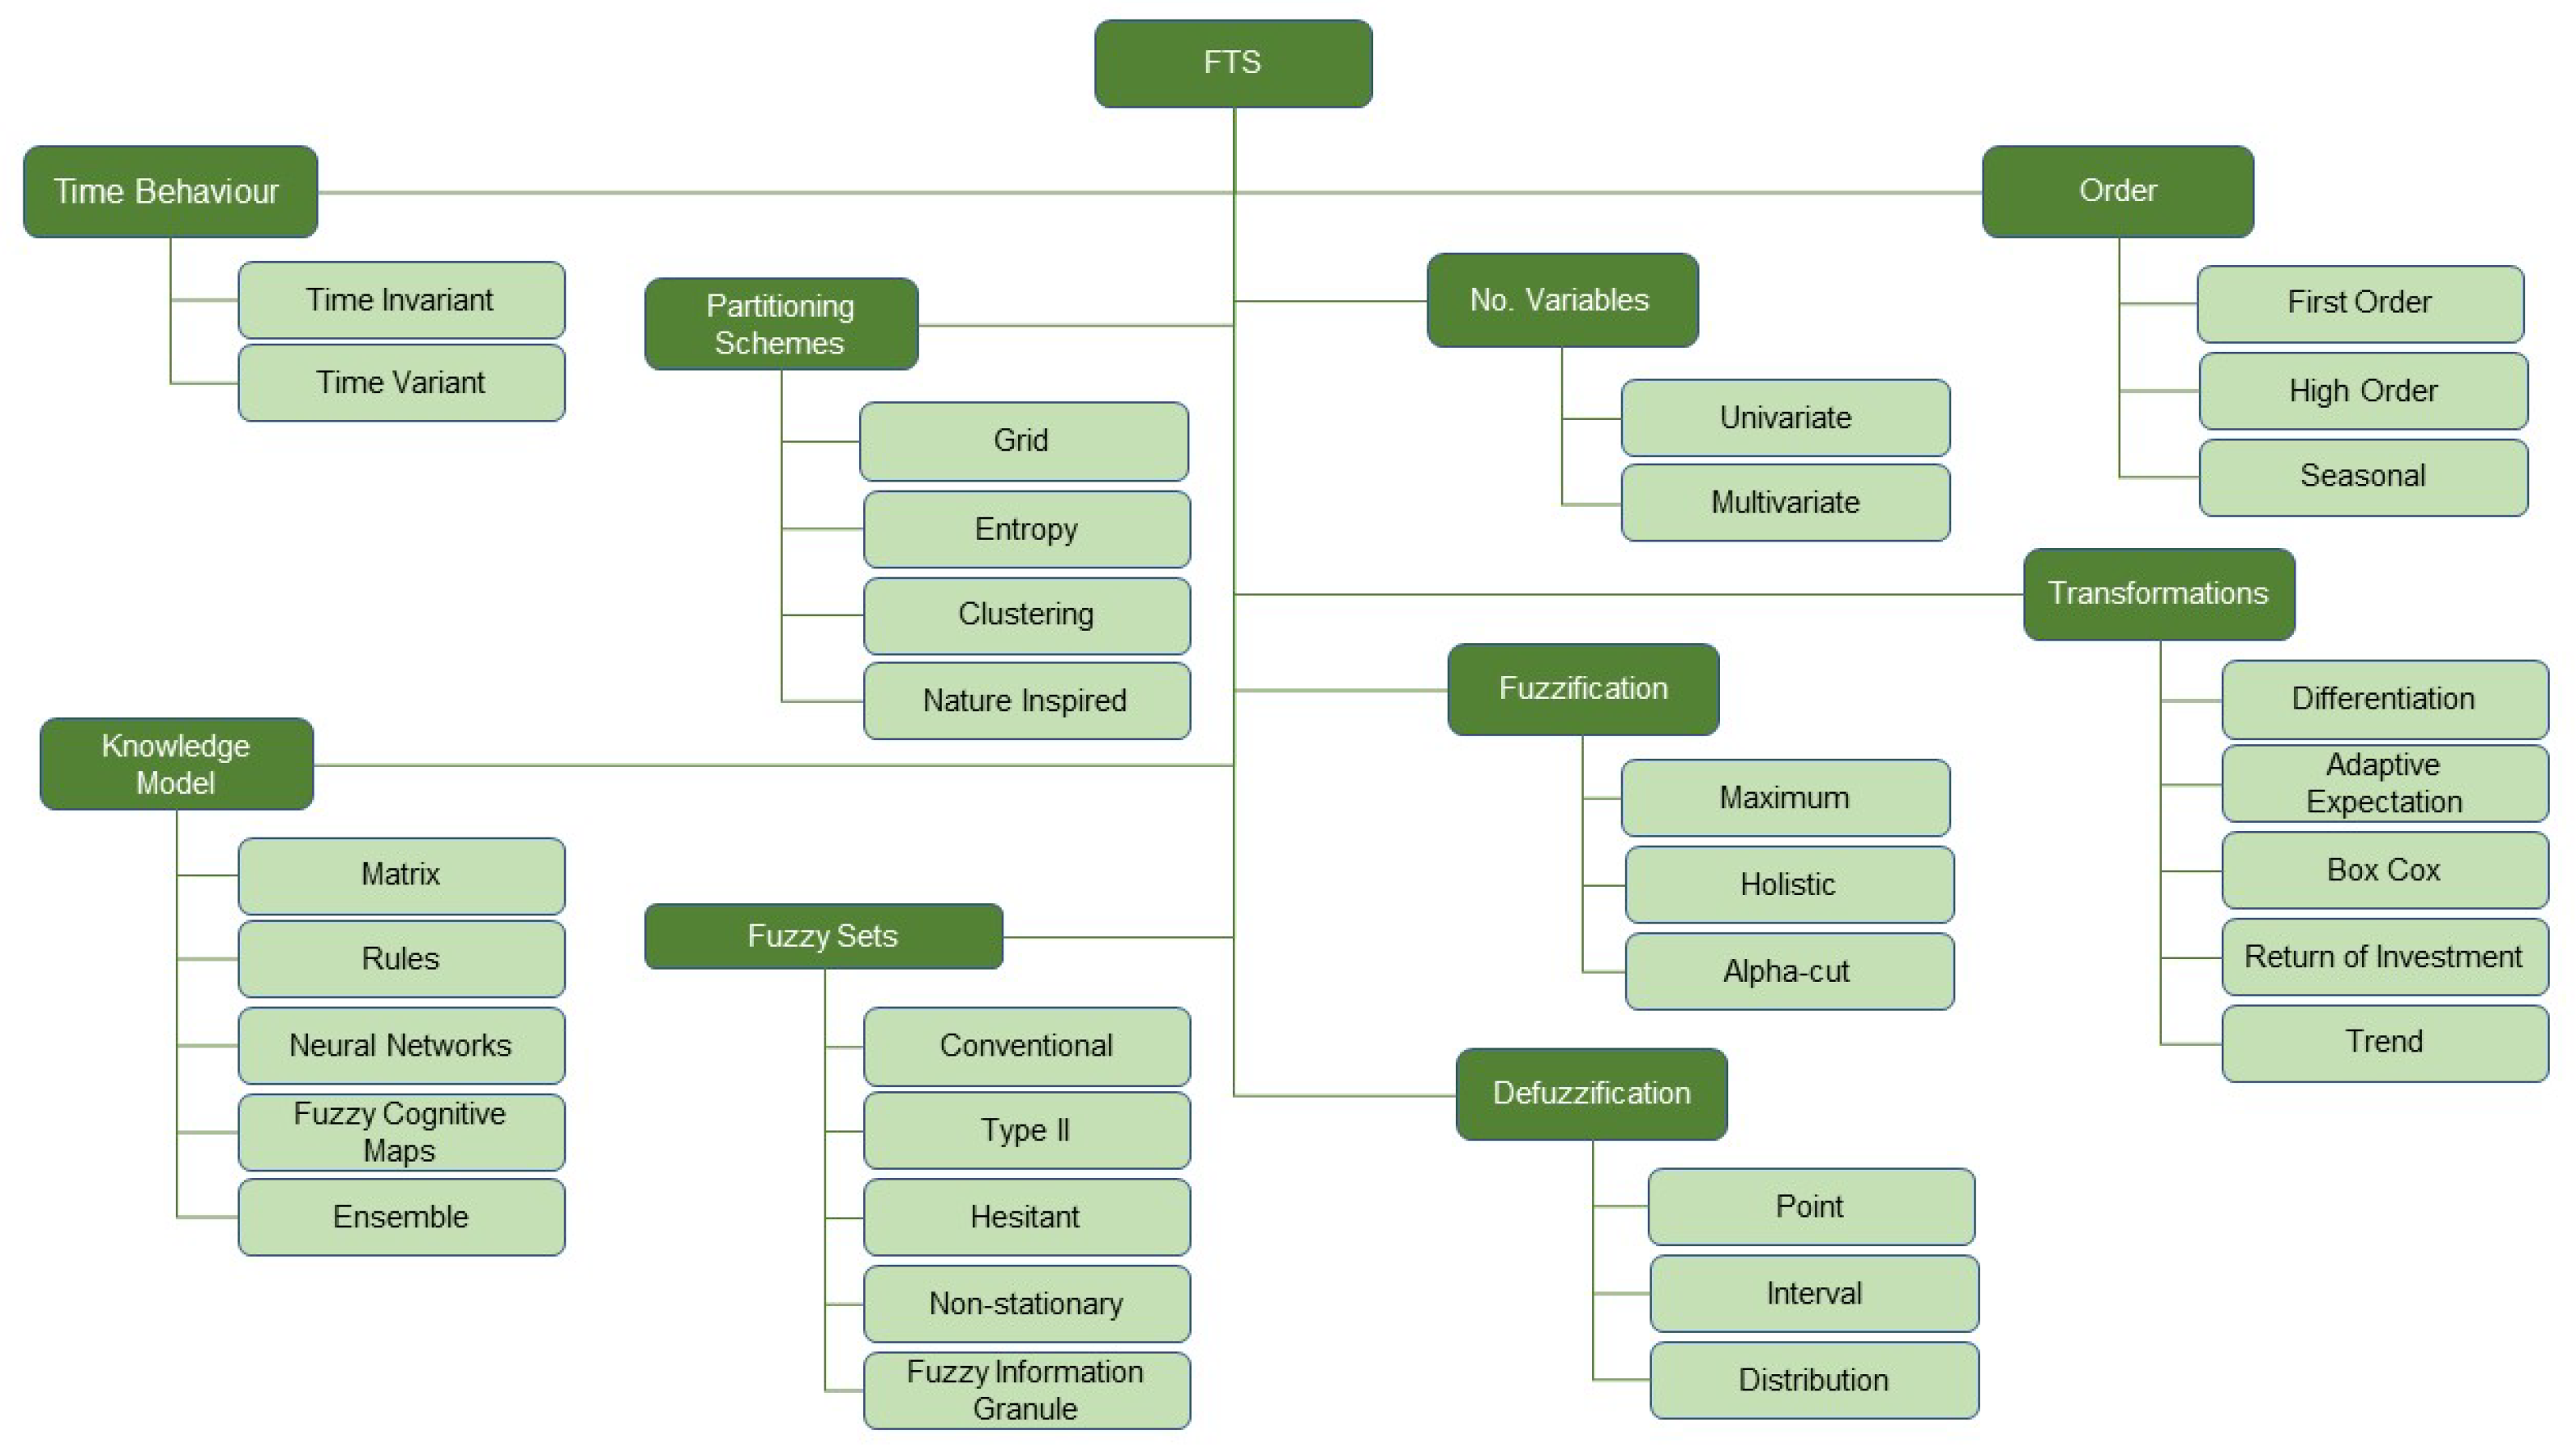
\includegraphics[width=1\linewidth]{Images/applsci-12-06894-g001.png}
		\end{figure}
	\end{frame}
	
	\begin{frame}{Santos Port — Time series characteristics}
		The Port of Santos plays an important maritime logistic hub for the international trade of Brazil. We can see by the table bellow that the main products that compose it's trades are part of the agricultural culture:
		
		\begin{table}[]
			\begin{tabular}{|l|l|}
				\hline
				Product	&  Tons \\ \hline
				Another Products	& 597.290.200 \\ \hline
				Sugar	& 372.621.400 \\ \hline
				Soybeans	& 347.725.600 \\ \hline
				Corn	& 210.871.300 \\\hline
				Soybean Meal	& 107.332.100 \\ \hline
				
			\end{tabular}
		\end{table}
		
		Another Products are a generic type of cargo that can mean anything else than the registered label of Santos Port Authority has assigned to their data.
		
	\end{frame}
	
	\begin{frame}{Santos Port Time Series}
		As we can see by the chart bellow, Santos Port cargo has an increasing total number of tons along the years.
		
		\begin{figure}
			\centering
			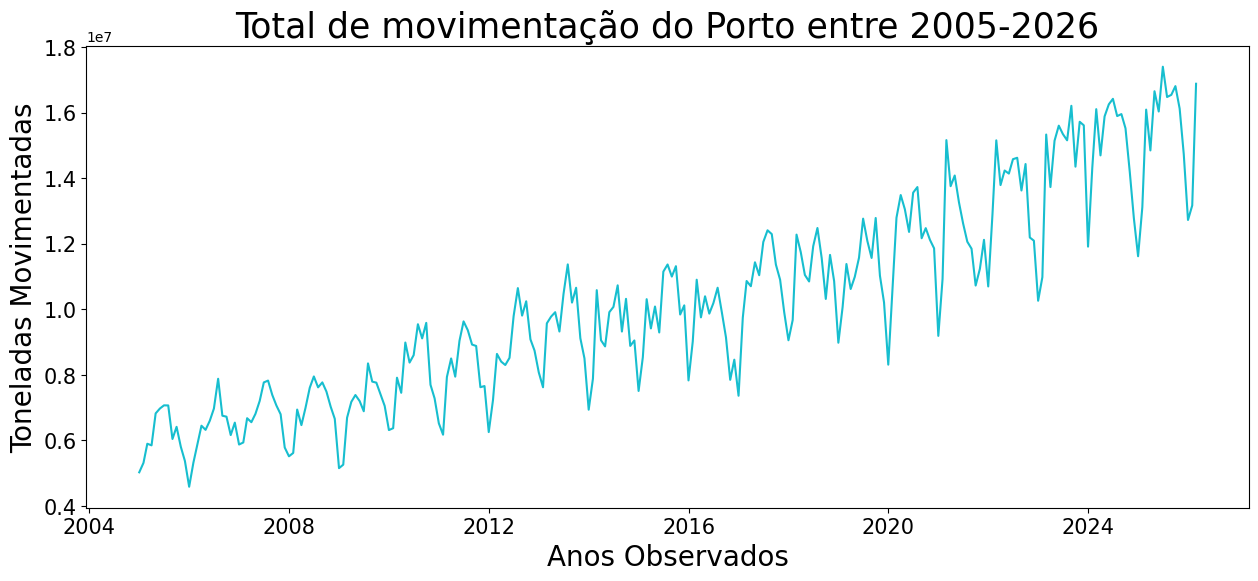
\includegraphics[width=1\linewidth]{Images/st_porto.png}
		\end{figure}
	\end{frame}
	
	\begin{frame}{Seasonality}
		The fact that Santos Port has mostly agricultural products, the harvest and off-season are strong manifested in the seasonality component.
		\begin{figure}
			\centering
			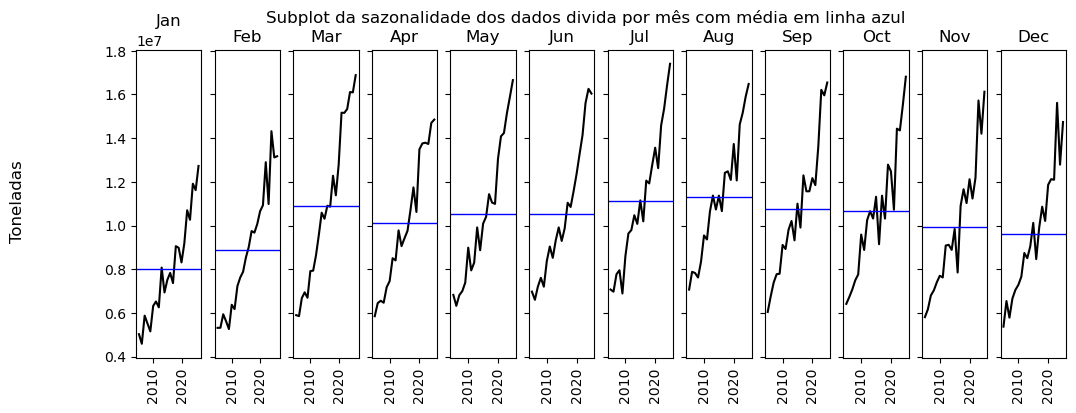
\includegraphics[width=1\linewidth]{Images/saz_porto.png}
		\end{figure}
	\end{frame}
	
	\begin{frame}{Trend}
		In this chart we have the trend-cycle component that follows an increasing trend over the years.
		\begin{figure}
			\centering
			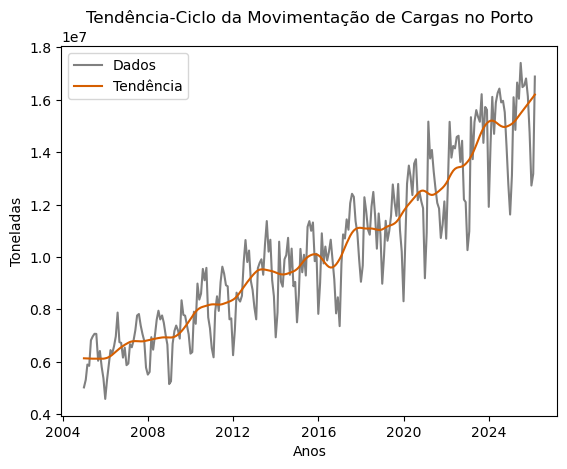
\includegraphics[width=1\linewidth]{Images/trend_porto.png}
		\end{figure}
	\end{frame}
	
	\begin{frame}{STL}
		Here we have the Seasonal Trend using Loess (STL) applied into the time series.
		\begin{figure}
			\centering
			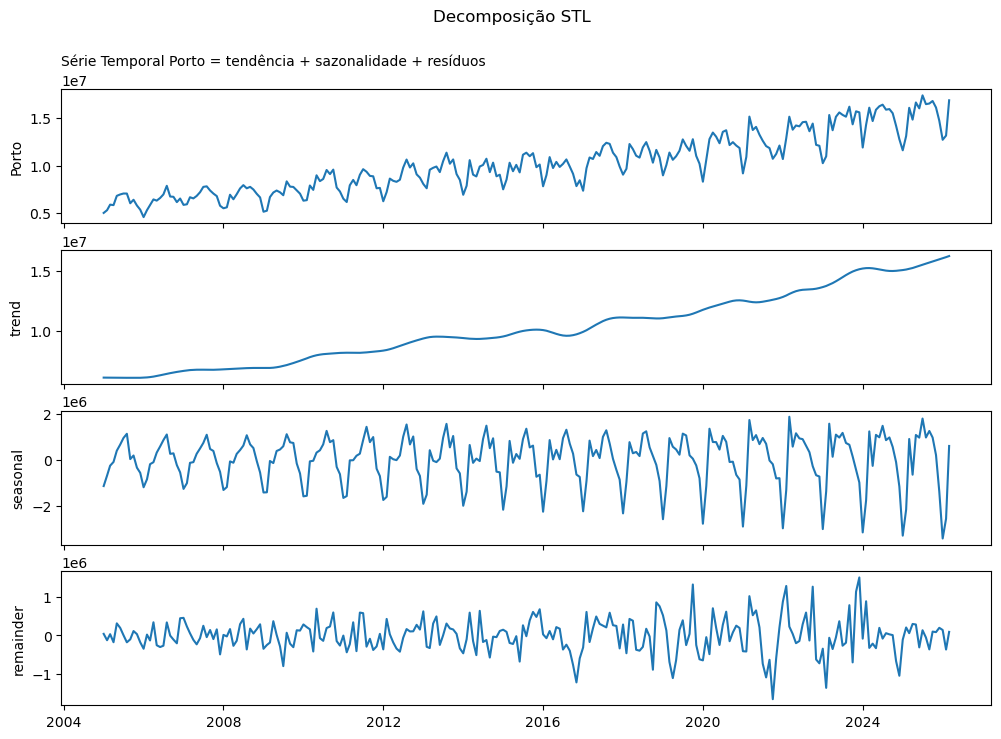
\includegraphics[width=1\linewidth]{Images/STL_porto.png}
		\end{figure}
	\end{frame}
	
	\begin{frame}{ACF, ADF and KPSS}
		The correlogram showed bellow is the measure of linear relationship between lagged values of a time series. It shows us in this scalloped format that this time series has an seasonal and trend composition. 
		\begin{figure}
			\centering
			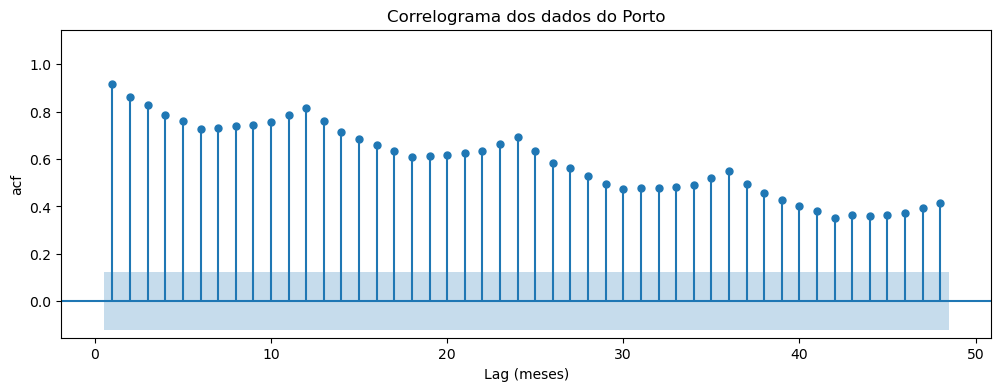
\includegraphics[width=1\linewidth]{Images/corr_porto.png}
		\end{figure}
		To formalize that the Argument Dickey-Fuller (ADF) and Kwiatkowski–Phillips–Schmidt–Shin (KPSS) are statistical test to confirm trend in a time series.
		$ ADF: p-value = 0.982791$ and $ KPSS: p-value =  0.01000$
	\end{frame}
	
	\begin{frame}{Fuzzy Time Series and Simple Linear Regression — What Your Model Assumes Before You Start.}
		
		Before we talk about this research, we are going to introduce a paper and one new concept. \newline
		
		The following paper is a general analysis about the cargo movement in Santos Port, with a forecasting using simple linear regression for 2023 to 2026:
		\textbf{Santos, Campos e Correa (2023). Santos Port
			Cargo handling analysis and future perspectives.}
		\newline
		
		The interesting thing about it is not only that applies another forecasting model into the same time series we were seeing, but also the linear regression model is one that assumes you have independently and identically distributed (iid) data. That for time series in special makes a model with necessary precautions and the same time one that most beginner statisticians are used to. 
		
	\end{frame}
	
	\begin{frame}
		\begin{columns}[T]
			\begin{column}{0.35\textwidth}
				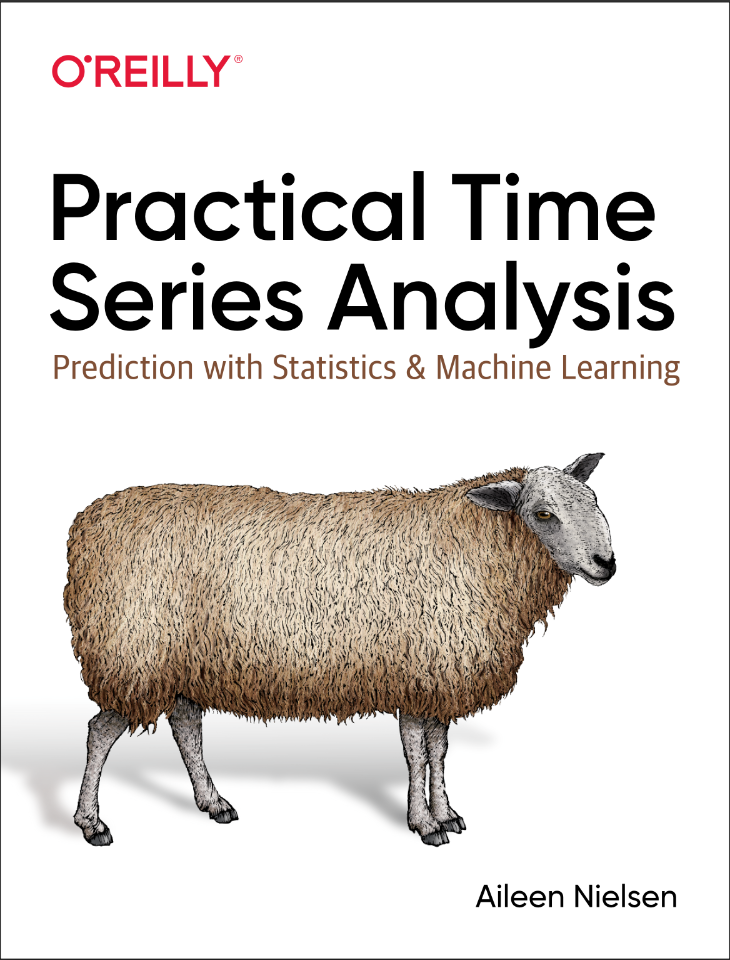
\includegraphics[width=\linewidth]{Images/PTSA}
				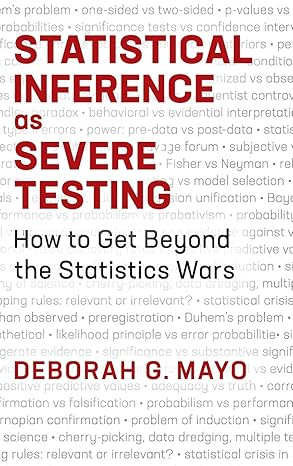
\includegraphics[width=\linewidth]{Images/Severe.jpg}
			\end{column}
			\begin{column}{0.60\textwidth}
				While Aileen Nielsen specify the assumptions due to the precautions with linear regression in time series data, she also says that real-world analysts usually take liberties in applying the model as long the trade-off from mathematical violations be worth it. (Which is the case we will see in the paper)
				\newline
				\newline
				Deborah Mayo exposes in her book these types of practices in the statistical field, where usually you have spurious application of models without the adequate testing. As she Denotes: Bad Evidence No Test (BENT) and the Misspecification of models.
			\end{column}
		\end{columns}
	\end{frame}
	
	\begin{frame}
		As in the current date of this research we already have some of the data from 2023 to 2026, we are going to see how the linear regression model visually performed in the period.
		
		\begin{figure}
			\centering
			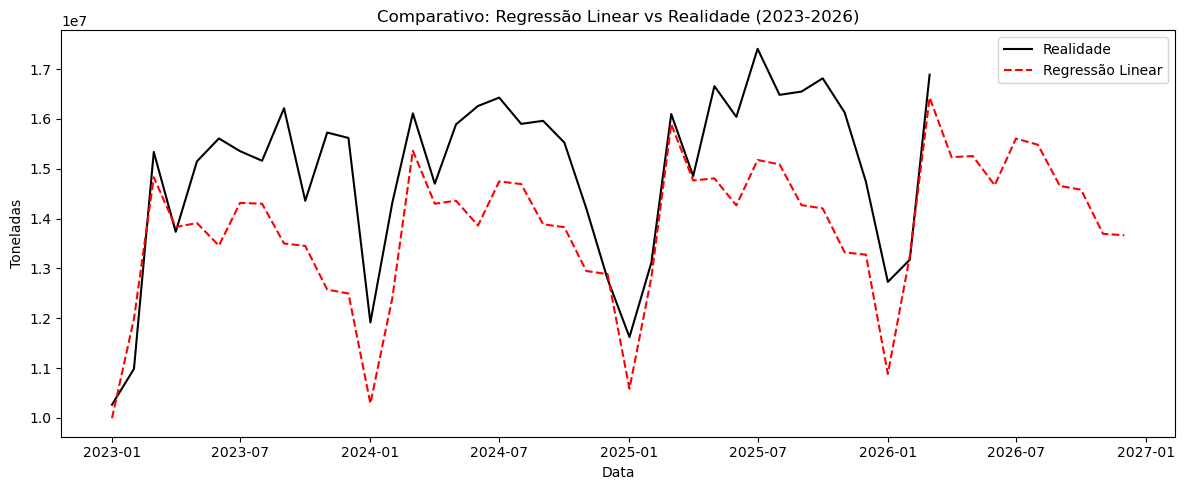
\includegraphics[width=\linewidth]{Images/real_rl.png}
		\end{figure}
		
		From what we can see the model has predicted well regarding some error after the peaks. Visually is clear that it has some accuracy and follows the data along time. But beyond the visual plot, there is a trade-off regarding it's assumptions as Aileen stated before.
		
	\end{frame}
	
	\begin{frame}
		In the paper we are discussing, the author's claimed that they choose to apply the linear regression model because offered a simple and easy to compute approach, and by that recognizing the limitations and indicating the SARIMA model for proper use in this time series. As they also stated in willing to use the simple linear regression it was necessary to train the model for each month in order to bypass the seasonality and generate the predictions.
		
		\begin{figure}
			\centering
			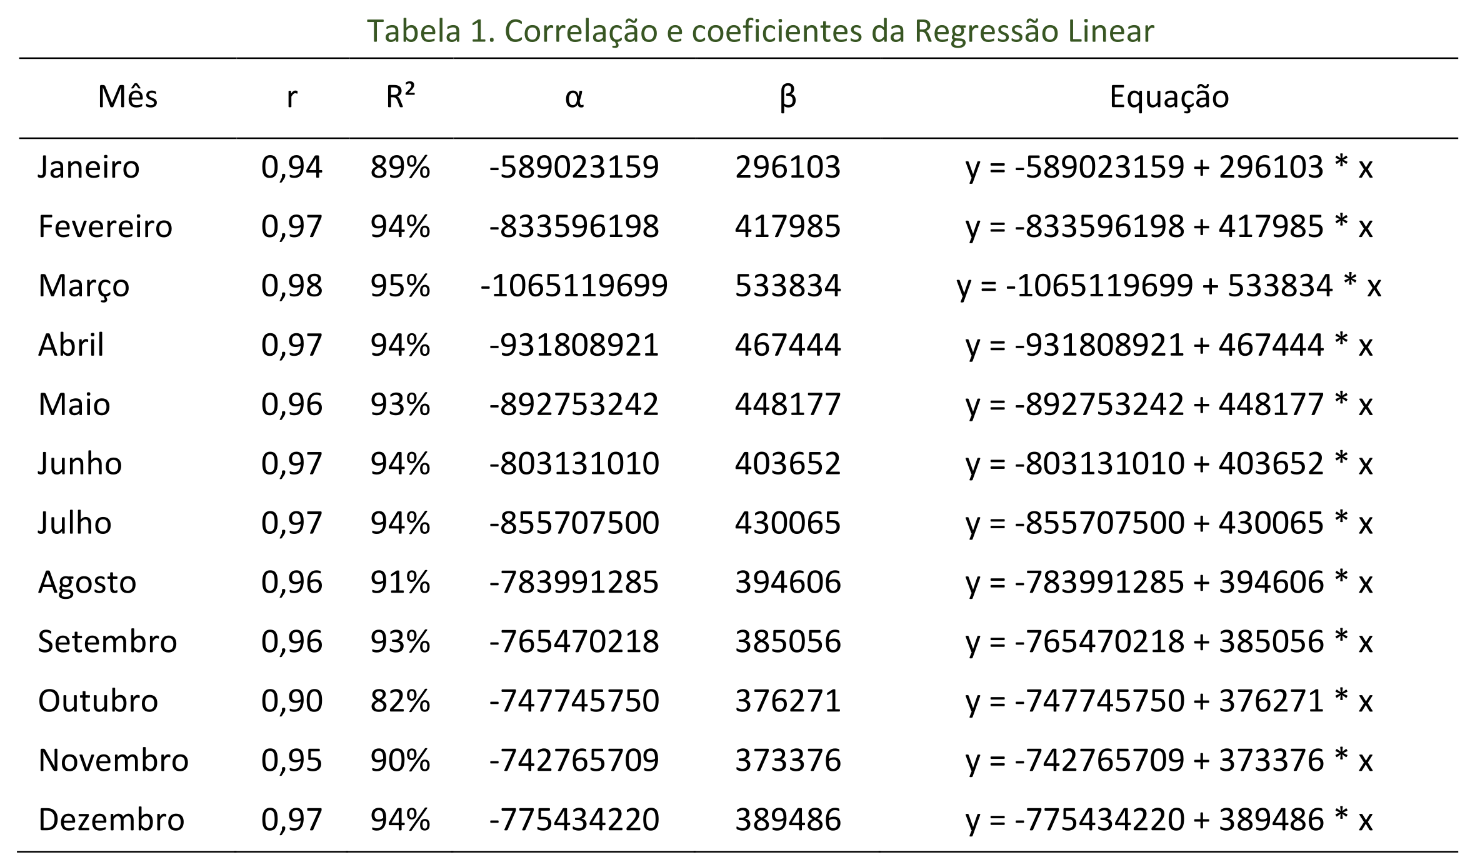
\includegraphics[width=0.8\linewidth]{Images/tabela.png}
		\end{figure}
		
	\end{frame}
	
	\begin{frame}
		Thus the problematic it implies that by slicing the model in 12 parts, 1 for each month, and fitting all those linear regression predictions into a whole forecasting is what Deborah Mayo exposed of the thoughtless pragmatics generating \textbf{BENT} and \textbf{Model Misspecification}.
		
		\begin{figure}
			\centering
			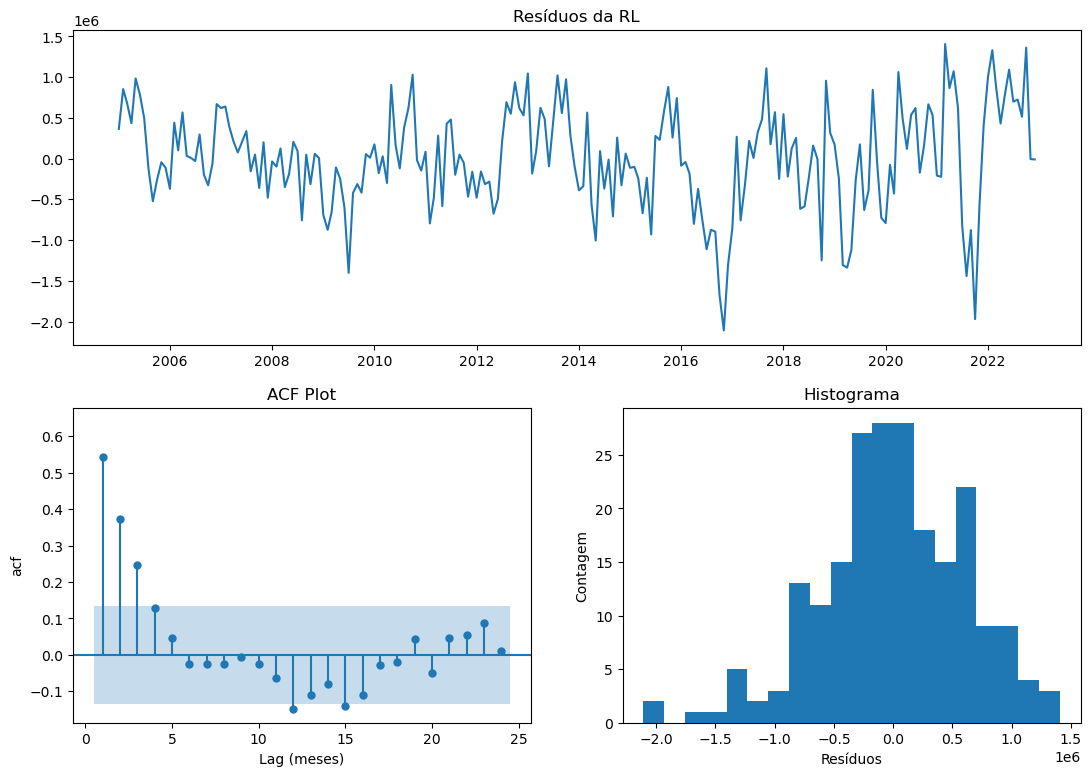
\includegraphics[width=\linewidth]{Images/diag_rl.png}
		\end{figure}   
		
	\end{frame}
	
	\begin{frame}
		
		\begin{figure}
			\centering
			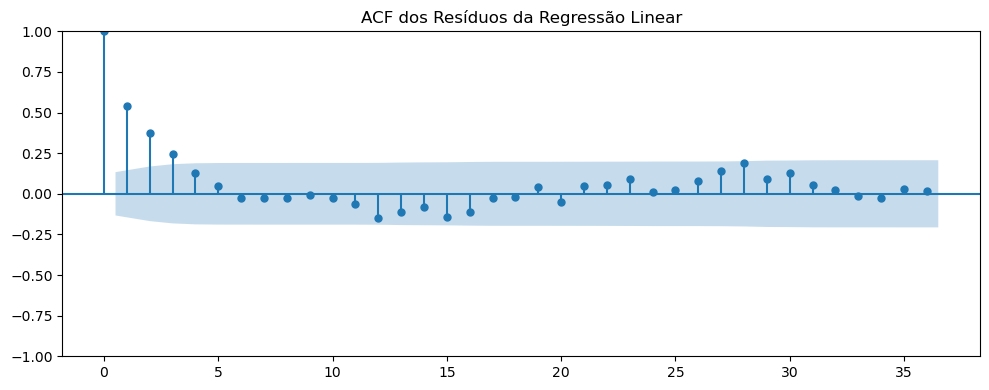
\includegraphics[width=\linewidth]{Images/resid_rl.png}
		\end{figure}
		
		By ACF from residuals we can immediate think of \textbf{White Noise}, after fitting a model and producing the predictions, we must confirm that nothing of valuable information remained at the residuals, in this case the ACF plot show us a pattern which is probably left by the bypassed seasonality and significant values in the lags [1, 2, 3] over the Confidence Interval. 
		
	\end{frame}
	
	\begin{frame}
		To formalize the visual information we need a statistical tests for checking autocorrelation present in the residual. One of them and widely use is the Lyung-Box test which states for $ H_0 $: the data is not correlated and $H_a:$ there is serial dependency (autocorrelation). 
		
		\vspace{0.5em}
		
		\begin{itemize}
			\setlength{\itemsep}{0.8em}
			\item \textbf{Ljung-Box} ($n = 216$, lags $= 12$): \\
			$\text{LB}_{12} = 119.27,\quad p = 8.6 \times 10^{-20}$
		\end{itemize}
		
		In our test it has giving us a $p-value = 0.00$ (rounded to 2 decimal case). Then we can reject the null hypothesis. 
		
	\end{frame}
	
	\begin{frame}{The Gauss-Markov Contract(Theorem)}
		
		Why all that formalism anyway? We clearly saw in the plot contrasting reality with foretasted values, the results where pretty close. \newline
		\newline
		Well, stochastic models are pretty good in terms of giving you a full hand of information when properly applied without breaking the premises. For the regression model \textbf{Gauss-Markov Theorem} states that by determined conditions the Ordinary Least Squared is:
		\begin{itemize}
			\item \textbf{B} est
			\item \textbf{L} inear
			\item \textbf{U} niased
			\item \textbf{E} stimator
		\end{itemize}
		therefore meaning that he has the lowest deviation (highest precision).
		
	\end{frame}
	
	\begin{frame}{Inference Problems}
		\begin{itemize}
			\item \textbf{Lying Inference} \newline
			With positive autocorrelation our standard error is affected to lowest value, this inflates the t-stat and make p-values look significant.\newline
			\item \textbf{High $R^2$} \newline
			The author's report high $R^2$ as a signal of good results in the model. But this can be problematic since in time series with autocorrelation the $R^2$ usually can be artificially high.\newline
			\item \textbf{Confidence Intervals} \newline
			As Rob Hyndman emphasizes the problem of bad inference, making a narrow confidence interval, which can affect major decisions giving the illusion of low risk in variance.
		\end{itemize}
	\end{frame}
	
	\begin{frame}{The Simplicity Argument}
		Until now we could see the problematic towards linear regression model, and we must know that is not prohibited to use linear regression in time series, but it is a special case where we must be attempt to the assumptions. \newline
		
		The claim of the linear regression was to make a "simple and cheap computational model" and "Avoid SARIMA", the only thing that maybe was missing is that Holt-Winters triple exponential smoothing is the perfect parametric model designed to handle a time series with trend and seasonality.
		
		\begin{columns}[T]
			
			\begin{column}{0.60\textwidth}
				\vspace{-6pt}
				\begin{align*}
					y_i &= \beta_0 + \beta_1 x_i + \varepsilon_i \\[4pt]
					\hat{\beta}_1 &= \frac{\sum_{i=1}^n (x_i - \bar{x})(y_i - \bar{y})}
					{\sum_{i=1}^n (x_i - \bar{x})^2} \\[4pt]
					\hat{\beta}_0 &= \bar{y} - \hat{\beta}_1\,\bar{x} \\[4pt]
					\hat{y}_i &= \hat{\beta}_0 + \hat{\beta}_1 x_i
				\end{align*}
			\end{column}
			
			\vrule{}
			
			\begin{column}{0.35\textwidth}
				\vspace{23pt}
				\scriptsize
				$\varepsilon_i \overset{\text{iid}}{\sim} \mathcal{N}(0,\sigma^2)$:
				Gauss--Markov assumptions\\[6pt]
				$\hat{y}_i$: fitted value\\[6pt]
				$\bar{x},\,\bar{y}$: sample means
			\end{column}
			
		\end{columns}
		
	\end{frame}
	
	\begin{frame}
		\begin{figure}
			\centering
			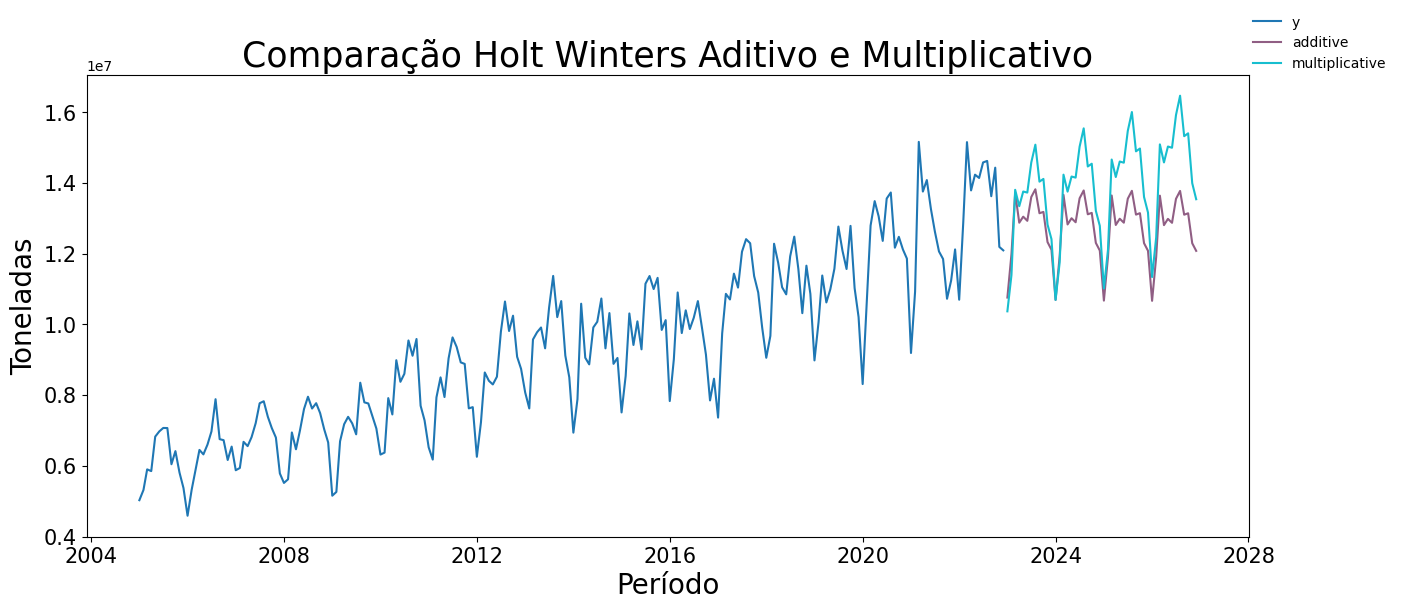
\includegraphics[width=1\linewidth]{Images/HW1.png}
		\end{figure}
		
		\footnotesize
		\begin{columns}[T]
			
			\begin{column}{0.48\textwidth}
				\centering
				\textbf{Additive}
				\begin{align*}
					\ell_t &= \alpha(y_t - s_{t-m})\\
					&\quad + (1-\alpha)(\ell_{t-1}+b_{t-1})\\
					b_t    &= \beta(\ell_t-\ell_{t-1})\\
					&\quad + (1-\beta)\,b_{t-1}\\
					s_t    &= \gamma(y_t-\ell_{t-1}-b_{t-1})\\
					&\quad + (1-\gamma)\,s_{t-m}\\[2pt]
					\hat{y}_{t+h} &= \ell_t + h\,b_t + s_{t-m+h_m^+}
				\end{align*}
			\end{column}
			
			\vrule{}
			
			\begin{column}{0.48\textwidth}
				\centering
				\textbf{Multiplicative}
				\begin{align*}
					\ell_t &= \alpha\,\frac{y_t}{s_{t-m}}\\
					&\quad + (1-\alpha)(\ell_{t-1}+b_{t-1})\\
					b_t    &= \beta(\ell_t-\ell_{t-1})\\
					&\quad + (1-\beta)\,b_{t-1}\\
					s_t    &= \gamma\,\frac{y_t}{\ell_{t-1}+b_{t-1}}\\
					&\quad + (1-\gamma)\,s_{t-m}\\[2pt]
					\hat{y}_{t+h} &= (\ell_t + h\,b_t)\cdot s_{t-m+h_m^+}
				\end{align*}
			\end{column}
			
		\end{columns}
		
	\end{frame}
	
	\begin{frame}{Holt-Winters}
		
		\begin{figure}
			\centering
			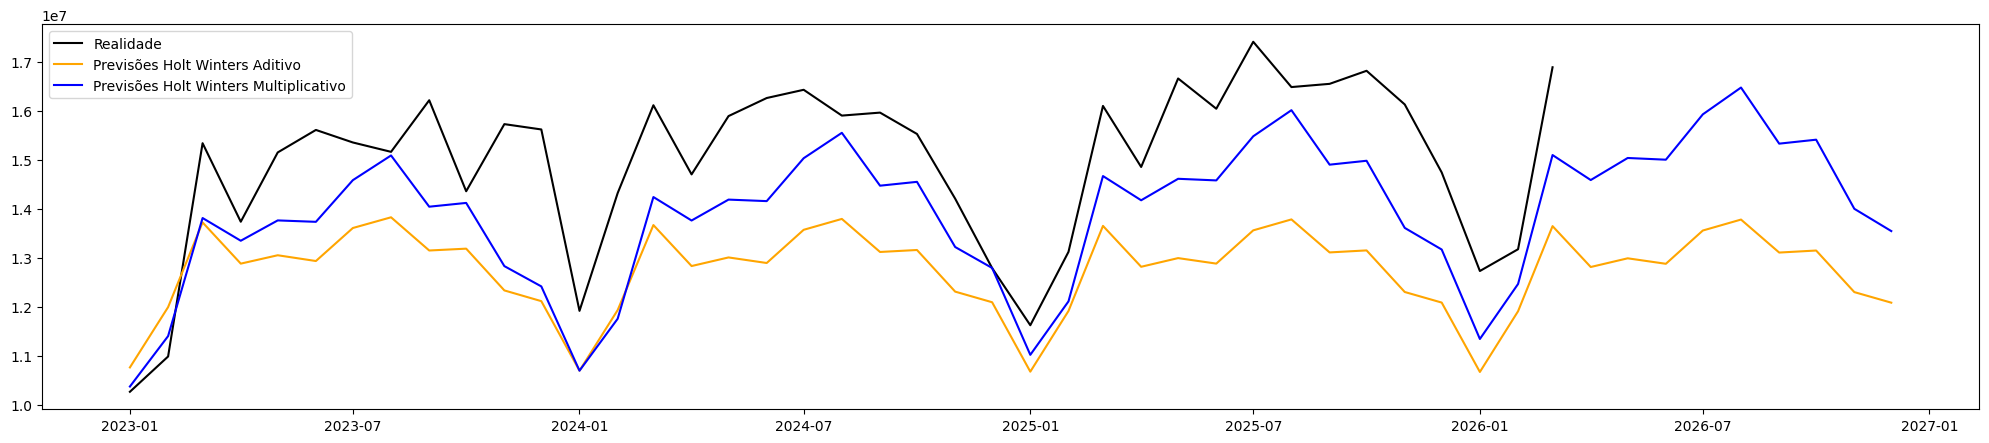
\includegraphics[width=1.2\linewidth]{Images/HW2.png}
		\end{figure}
		
		\begin{columns}[T]
			\begin{column}{0.6\textwidth}
				\begin{figure}
					\centering
					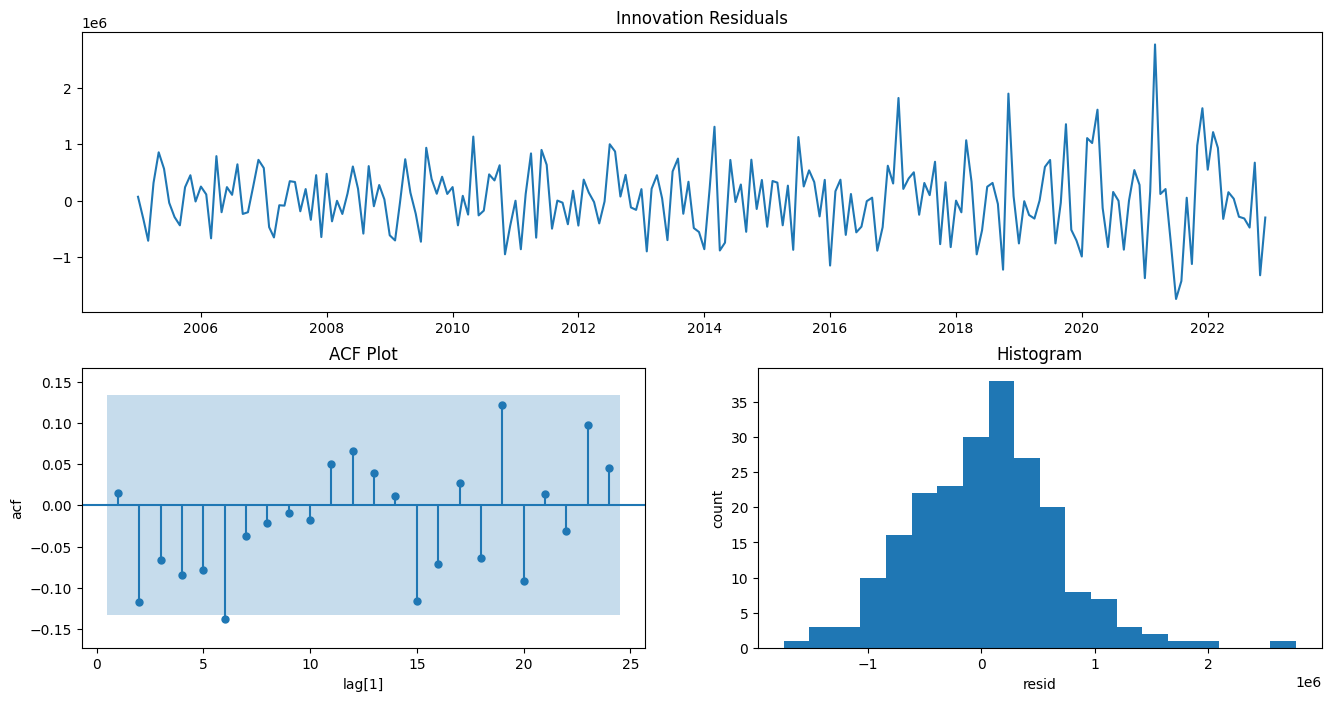
\includegraphics[width=1\linewidth]{Images/HWadd_res.png}
				\end{figure}
				$[0.821508,  0.080154, 0.342379]$
			\end{column}
			
			\begin{column}{0.6\textwidth}
				\begin{figure}
					\centering
					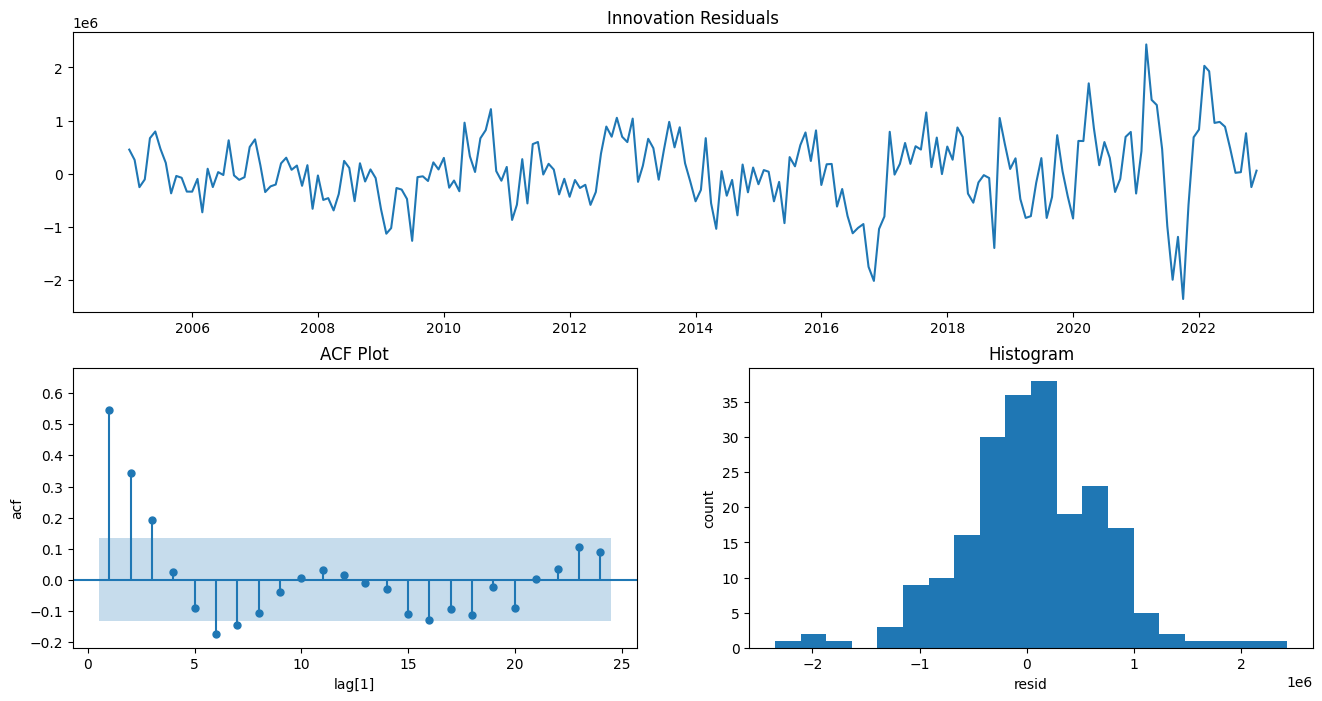
\includegraphics[width=1\linewidth]{Images/HWmul_respng.png}
				\end{figure}
				$[0.0, 0.0, 0.0]$
			\end{column}
		\end{columns}
		
	\end{frame}
	
	\begin{frame}{Seasonal Naïve}
		
		Considering that we doesn't care about the residuals of the model and we search for the simplest way to prospect future values, how could we do it? Well, instead of trying to bypassing seasonality we use it as our main predictor:
		
		\begin{figure}
			\centering
			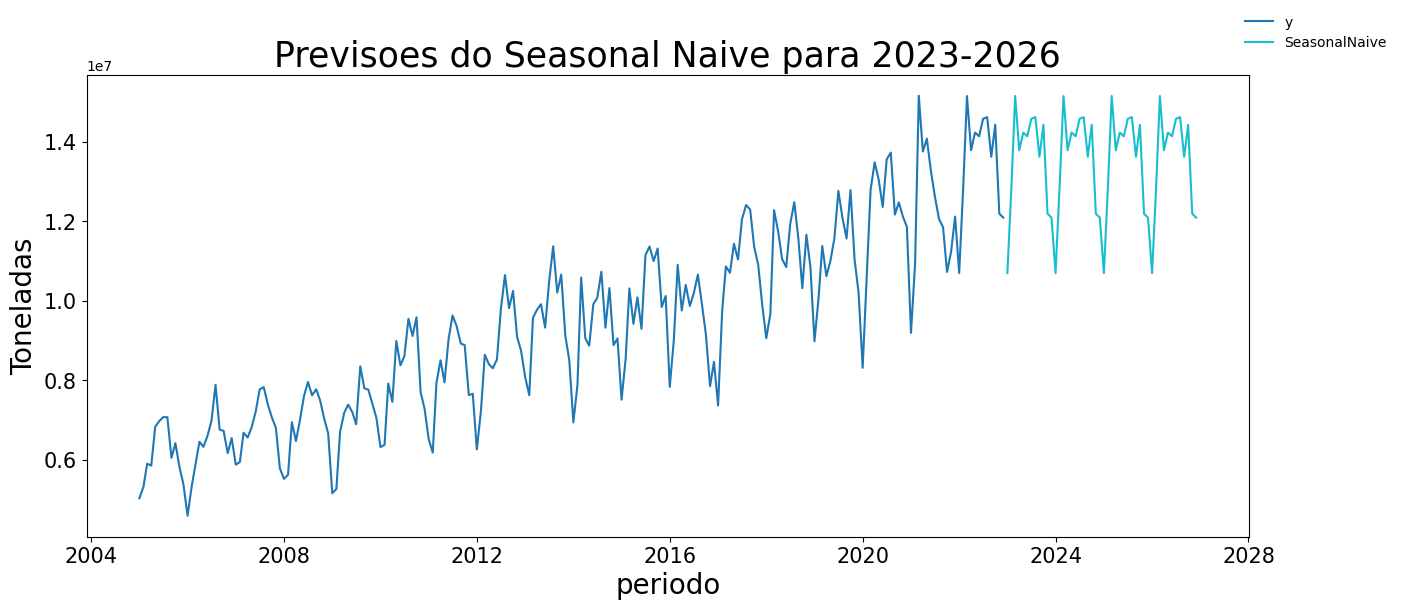
\includegraphics[width=1\linewidth]{Images/Snad.png}
		\end{figure}
		
	\end{frame}
	
	\begin{frame}{Seasonal Naïve and Linear Regression}
		
		Here we can see that the Seasonal Naïve stays very close to the Linear Regression model. The RMSE and MAPE reveals that Seasonal Naïve performs worse in both metrics with a small difference, this is because the Time Series is compose strongly by Season but also Trend-Cycle and remainders that it fails to captures. While the pure linear regression can mimic the seasonal patter and adsorb the trend component.
		
		\begin{figure}
			\centering
			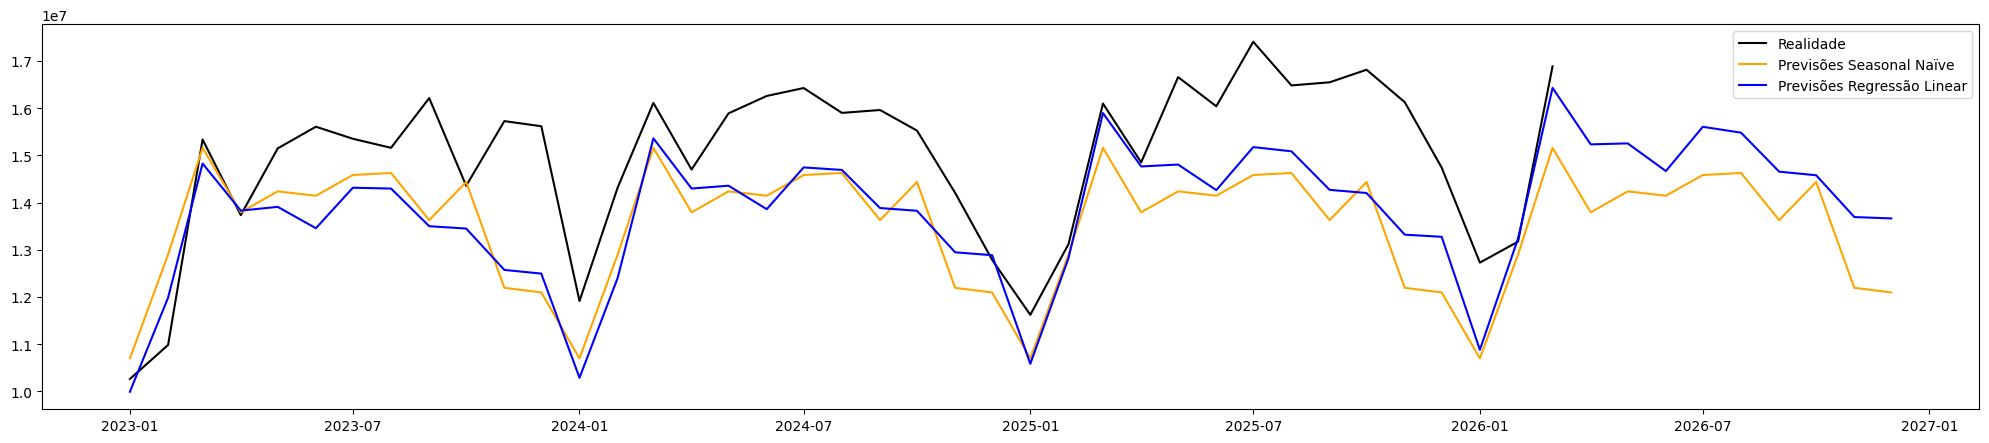
\includegraphics[width=1.2\linewidth]{Images/Snad_RL.png}
		\end{figure}
		
		\vspace{-4pt}
		\centering
		\footnotesize
		\begin{tabular}{lcc}
			\hline
			\textbf{Model} & \textbf{RMSE} & \textbf{MAPE (\%)} \\
			\hline
			Seasonal Naïve       & 1{,}863{,}004.16 & 10.34 \\
			Linear Regression    & 1{,}646{,}719.79 &  9.09 \\
			\hline
		\end{tabular}
		
	\end{frame}
	
	\begin{frame}{Axiomatic Structures of Metamathematics}
		
		\begin{columns}[T]
			
			\begin{column}{0.60\textwidth}
				\footnotesize
				A scientific theory is not merely a collection of concepts —
				it is \textbf{structured conceptual knowledge} embedded in a
				metamathematical framework.
				\textbf{Krause (2022)} argues that models of scientific theories
				are set-theoretical entities, and the choice of the underlying
				set theory is not neutral: it constrains what the model
				can express, infer, and guarantee.
				
				\vspace{6pt}
				Two foundational positions:
				\begin{itemize}
					\scriptsize
					\item[\textbullet] \textbf{van Fraassen}: \textit{"To present a
						theory is to specify a family of structures, its models"}
					\item[\textbullet] \textbf{Suppes}: \textit{"A possible realization
						of a theory is a set-theoretical entity of the appropriate
						logical type"}
				\end{itemize}
				
				\vspace{6pt}
				\footnotesize
				Applying a model \textbf{outside} its axiomatic structure produces
				what Mayo calls \textbf{BENT} — inference without an honest test.
			\end{column}
			
			\vrule{}
			
			\begin{column}{0.35\textwidth}
				\begin{figure}
					\centering
					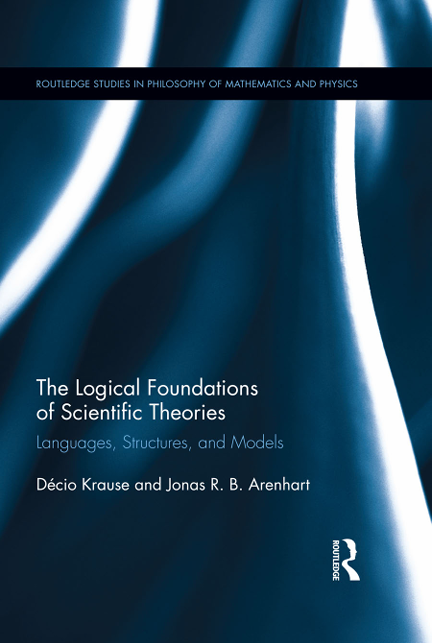
\includegraphics[width=1.1\linewidth]{Images/Krause.png}
				\end{figure}
			\end{column}
			
		\end{columns}
		
	\end{frame}
	
	\begin{frame}{Chen FTS}
		\begin{figure}
			\centering
			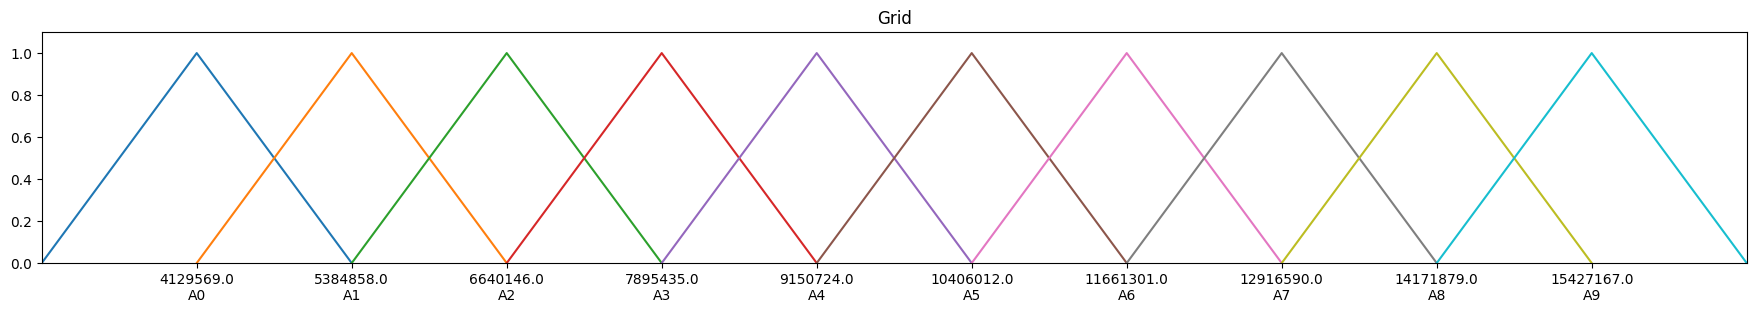
\includegraphics[width=1\linewidth]{Images/Chen_grid.png}
		\end{figure}
		\begin{figure}
			\centering
			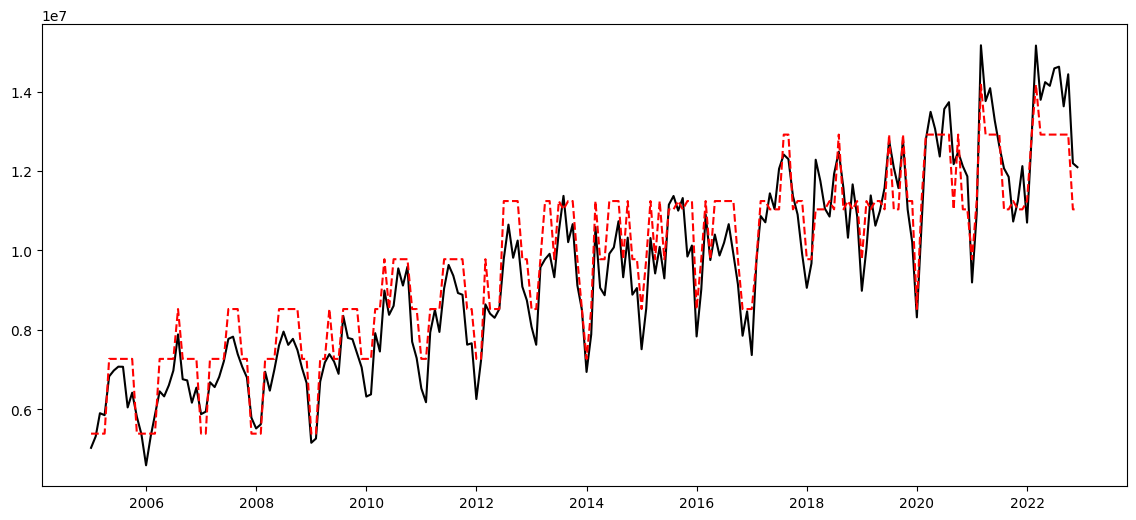
\includegraphics[width=1\linewidth]{Images/Chen_In_Sample.png}
		\end{figure}
	\end{frame}
	
	\begin{frame}{Point Forecast}
		\begin{figure}
			\centering
			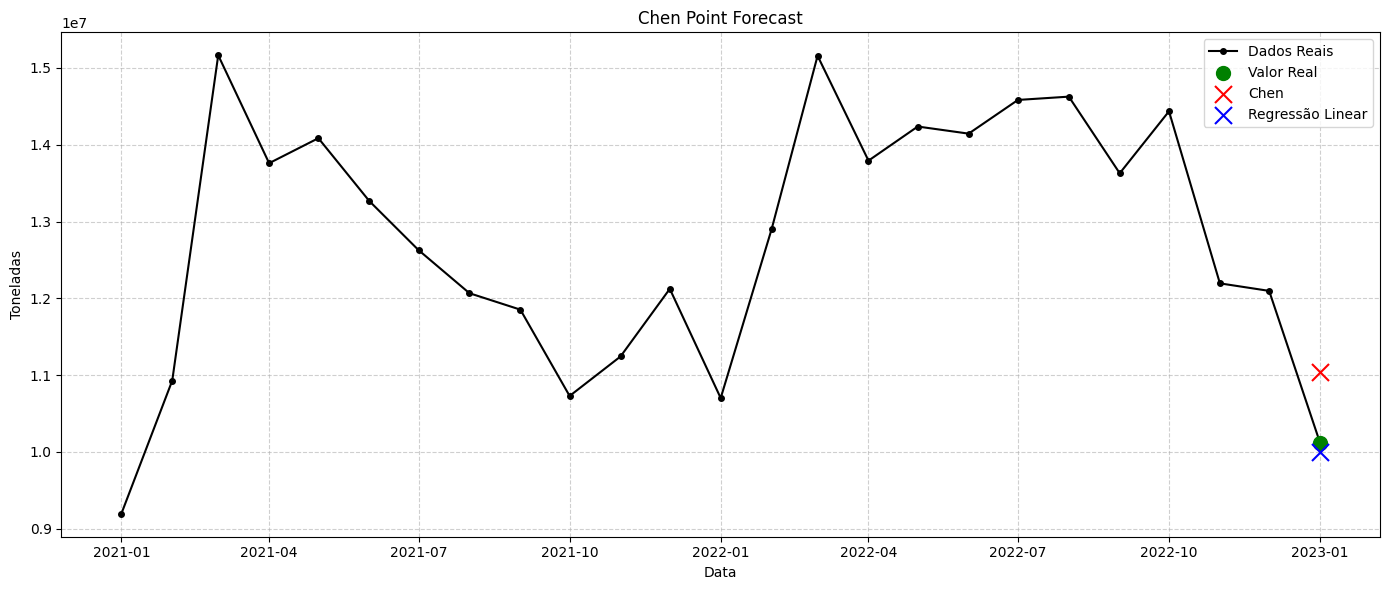
\includegraphics[width=1\linewidth]{Images/Chen_Point.png}
		\end{figure}
		
	\end{frame}
	
	\begin{frame}{The Axiomatic Honesty}
		In our case, we adopted the challenge to apply a simple model in the complex seasonal trended time series from Santos Port. While in the fundamentals aspect we thought that would be a interesting case to revoke linear or exponential models and adopt a shift in modeling the series with Fuzzy Time Series. The preliminary results are shown bellow:
		
		\begin{figure}
			\centering
			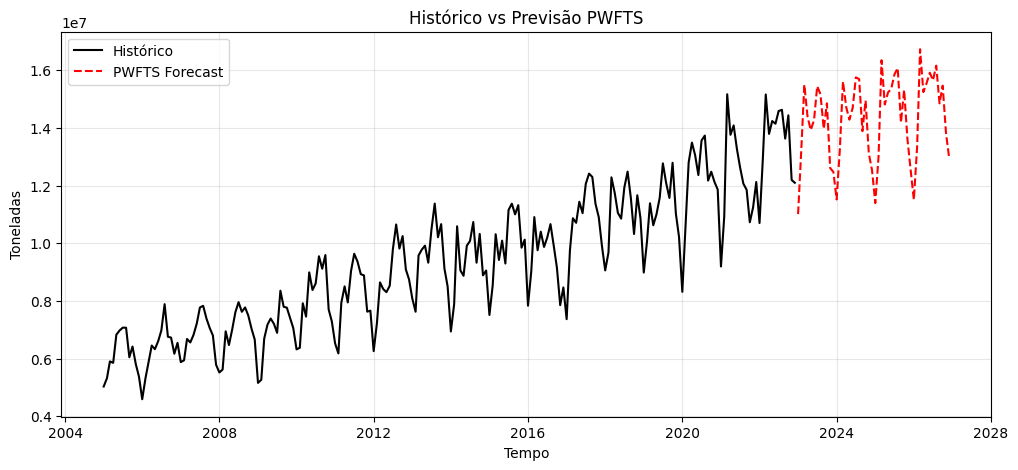
\includegraphics[width=\linewidth]{Images/PWFTS.png}
		\end{figure}	
	\end{frame}
	
	\begin{frame}{}
		While the FTS model has no inferences, just as the misspecified linear regression, we argue that he is "axiomatic honest" due to not violate his subjacent structure. 
		\begin{figure}
			\centering
			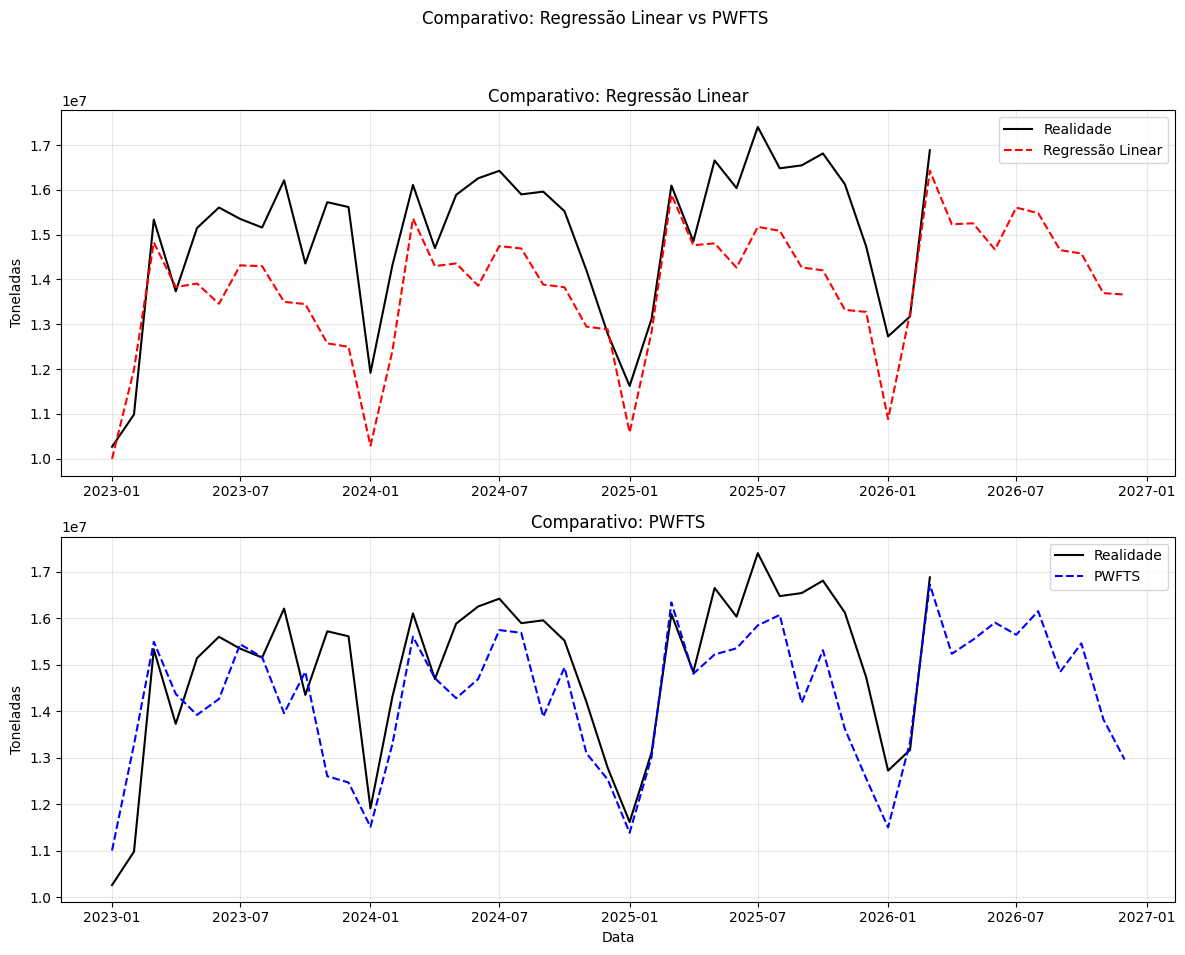
\includegraphics[width=1\linewidth]{Images/PWFTS_RL.png}
		\end{figure}
	\end{frame}
	
	\begin{frame}{Hybrid PWFTS and Seasonal Naïve}
		
		\begin{figure}
			\centering
			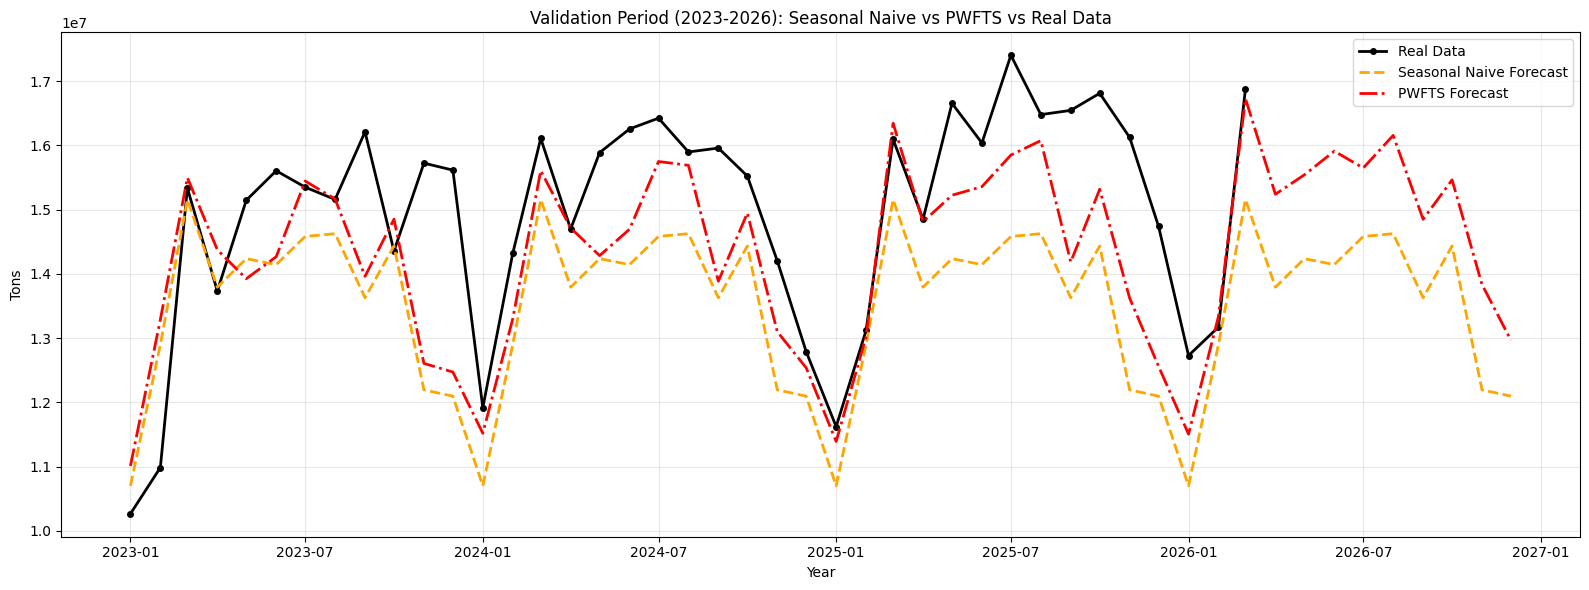
\includegraphics[width=\linewidth]{Images/PWFTS_SNAD.png}
		\end{figure}
		
	\end{frame}
	
	\begin{frame}{The End}
		\centering{\Huge{That's it, thanks for watching!}}
	\end{frame}
	
\end{document}